\subsection{RAID}
Redundant array of independent disks (RAID) is designed as a visualization tool that construct a single storage space with multiple disks. In a RAID system, a file is stripped and stored in different physical disks. A number of variations are evolved to provide different level of data redundancy and I/O performance enhancement \cite{arpaci2012operating}. These variations are \textit{levels}, known as 'RAID' followed by a level number. For example, the most common types of RAID are RAID-0, RAID-1 to RAID-6. Different levels of RAID are differ in their strategies in file striping, mirroring and parity computation. We focus on RAID-6 in this paper.

As a significant advantage compared to the lower levels, RAID-6 is resilient to two arbitrarily disk failure. To be more specific, it is capable of carrying on read and write request to any logic disk despite any two of them are not accessible. Figure \ref{fig:raid6} shows an example of a RAID 6 storage system with data blocks $A, B, C, D$ and $E$, each block is stripped into three parts (1-3) and two parities $p$ and $q$. 

\begin{figure}[t]
	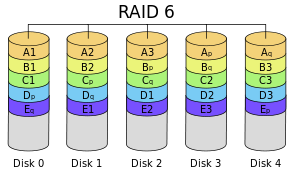
\includegraphics[width=9cm,height=5cm,angle=0]{RAID6.png}
	\caption{Diagram of a RAID 6 storage system with 3 block level data strippings and 2 parities \cite{wiki:raid} }
	\label{fig:raid6}
\end{figure}

In Red Hat Linux operating system's kernel implements RAID-6 for fault-tolerance, where the parities are computed as shown in Equation \ref{eq:1}:

\begin{equation} \label{eq:1}
\begin{array}{lcr} p = d_0 \oplus d_1 \oplus ... \oplus d_{k-1} \\
q = d_0 \oplus 2(d_1) \oplus ... \oplus 2^{k-1}(d_{k-1}) 
\end{array}
\end{equation}

The arithmetic operates in Galois field $GF(2^8)$, where addition $\oplus$ is equivalent to XOR and multiplication is more complicated but all results are found in a closed set from 0 to $2^8$. An interesting property about parity $q$ is that its computation can be transformed using only addition and multiplication by two, i.e. $q = 2 (2(...2(2d_{k-1} \oplus d_{k-2})...) \oplus d_1) \oplus d_0$, benefiting from efficient vector computation tricks in hardware.




\subsection{Erasure Coding}

Erasure coding is the technique used to compute the parities in RAID. It encodes data into data plus codings, so the original contents are recoverable when disks with data fail. More formally, for a given $k$ disks space of data, erasure coding creates $k+m$ disks of data, where $m$ disks are codings or parities. In the best case, the contents are recoverable by decoding the erasure code when up to $m$ disks failed. This optimality is called \textit{maximum distance
separable} (MDS). In the example from Figure \ref{fig:raid6}, a specific erasure coding algorithm can be used to calculate from three disks of data to produce $3+2=5$ disks of data and stored in five disks, where parities $p$ and $q$ are codings information that is essential for data recovery. If the encoding can recover data despite of an arbitrary two disks failure, the coding is MDS. 

In the example, parities are being stored in all available disks with each stripe rotates the identities of the disks . A more common alternative is to store $p$ segments and $q$ segments in two disks separated from the data parts, this is called a systematic coding.


%\subsection{Galois field}
%The first parity in RAID 6 is usually computed with a $XOR$ operation, while the other is preferred to be computed in a Galois field. Galois Field is a finite field that the size of membership is limited to $p^k$, where $p$ is a prime number and $k$ is a positive integer. 
%
%For example, the range of valid numbers in a Galois field $GF(2^8)$ is $0$ to $2^8-1=255$, and the 


\subsection{Reed-Solomen Coding}

A popular erasure coding scheme is Reed--Solomon coding. It was used for Linux RAID-6, Windows Azure Cloud storage and many other production systems. An \textit{encoding matrix}, or \textit{Generator Matrix} is used to achieve the encoding. Figure \ref{fig:encoding_matrix} shows an encoding matrix used in Linux RAID-6 for (6+2) erasure coding. The encoding is dot product of the encoding matrix and data vector. Noted that the top square matrix is an identity matrix, ensuring the first $k$ blocks are identical to the data blocks, here $k=6$. The last two rows of the matrix are implementation of Equation \ref{eq:1} to compute parities $p$ and $q$.

Vandermonde matrix is 


\begin{figure}[t]
	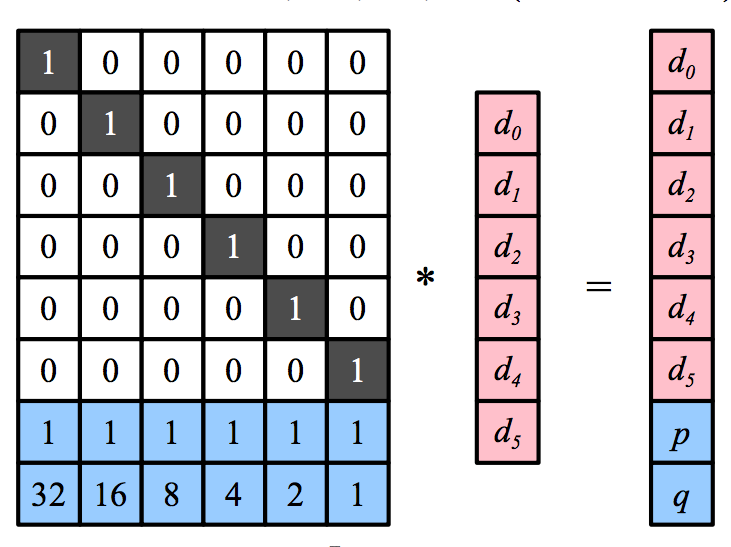
\includegraphics[width=8cm,height=5cm,angle=0]{encoding_matrix.png}
	\caption{An encoding matrix used in Linux RAID-6 with 6 data disks and 2 parities $(6,4)$ \cite{plank2013tutorial} }
	\label{fig:encoding_matrix}
\end{figure}


In this paper, we implement a RAID-6 based erasure coding by rewriting Reed--Solomen coding algorithm.
